\documentclass[]{article}
\usepackage{lmodern}
\usepackage{amssymb,amsmath}
\usepackage{ifxetex,ifluatex}
\usepackage{fixltx2e} % provides \textsubscript
\ifnum 0\ifxetex 1\fi\ifluatex 1\fi=0 % if pdftex
  \usepackage[T1]{fontenc}
  \usepackage[utf8]{inputenc}
\else % if luatex or xelatex
  \ifxetex
    \usepackage{mathspec}
  \else
    \usepackage{fontspec}
  \fi
  \defaultfontfeatures{Ligatures=TeX,Scale=MatchLowercase}
\fi
% use upquote if available, for straight quotes in verbatim environments
\IfFileExists{upquote.sty}{\usepackage{upquote}}{}
% use microtype if available
\IfFileExists{microtype.sty}{%
\usepackage{microtype}
\UseMicrotypeSet[protrusion]{basicmath} % disable protrusion for tt fonts
}{}
\usepackage[margin=1in]{geometry}
\usepackage{hyperref}
\hypersetup{unicode=true,
            pdftitle={Survey Data Analysis Final Report},
            pdfauthor={Sanne Meijering; Hanne Oberman; Gerbrich Ferdinands},
            pdfborder={0 0 0},
            breaklinks=true}
\urlstyle{same}  % don't use monospace font for urls
\usepackage{color}
\usepackage{fancyvrb}
\newcommand{\VerbBar}{|}
\newcommand{\VERB}{\Verb[commandchars=\\\{\}]}
\DefineVerbatimEnvironment{Highlighting}{Verbatim}{commandchars=\\\{\}}
% Add ',fontsize=\small' for more characters per line
\usepackage{framed}
\definecolor{shadecolor}{RGB}{248,248,248}
\newenvironment{Shaded}{\begin{snugshade}}{\end{snugshade}}
\newcommand{\KeywordTok}[1]{\textcolor[rgb]{0.13,0.29,0.53}{\textbf{#1}}}
\newcommand{\DataTypeTok}[1]{\textcolor[rgb]{0.13,0.29,0.53}{#1}}
\newcommand{\DecValTok}[1]{\textcolor[rgb]{0.00,0.00,0.81}{#1}}
\newcommand{\BaseNTok}[1]{\textcolor[rgb]{0.00,0.00,0.81}{#1}}
\newcommand{\FloatTok}[1]{\textcolor[rgb]{0.00,0.00,0.81}{#1}}
\newcommand{\ConstantTok}[1]{\textcolor[rgb]{0.00,0.00,0.00}{#1}}
\newcommand{\CharTok}[1]{\textcolor[rgb]{0.31,0.60,0.02}{#1}}
\newcommand{\SpecialCharTok}[1]{\textcolor[rgb]{0.00,0.00,0.00}{#1}}
\newcommand{\StringTok}[1]{\textcolor[rgb]{0.31,0.60,0.02}{#1}}
\newcommand{\VerbatimStringTok}[1]{\textcolor[rgb]{0.31,0.60,0.02}{#1}}
\newcommand{\SpecialStringTok}[1]{\textcolor[rgb]{0.31,0.60,0.02}{#1}}
\newcommand{\ImportTok}[1]{#1}
\newcommand{\CommentTok}[1]{\textcolor[rgb]{0.56,0.35,0.01}{\textit{#1}}}
\newcommand{\DocumentationTok}[1]{\textcolor[rgb]{0.56,0.35,0.01}{\textbf{\textit{#1}}}}
\newcommand{\AnnotationTok}[1]{\textcolor[rgb]{0.56,0.35,0.01}{\textbf{\textit{#1}}}}
\newcommand{\CommentVarTok}[1]{\textcolor[rgb]{0.56,0.35,0.01}{\textbf{\textit{#1}}}}
\newcommand{\OtherTok}[1]{\textcolor[rgb]{0.56,0.35,0.01}{#1}}
\newcommand{\FunctionTok}[1]{\textcolor[rgb]{0.00,0.00,0.00}{#1}}
\newcommand{\VariableTok}[1]{\textcolor[rgb]{0.00,0.00,0.00}{#1}}
\newcommand{\ControlFlowTok}[1]{\textcolor[rgb]{0.13,0.29,0.53}{\textbf{#1}}}
\newcommand{\OperatorTok}[1]{\textcolor[rgb]{0.81,0.36,0.00}{\textbf{#1}}}
\newcommand{\BuiltInTok}[1]{#1}
\newcommand{\ExtensionTok}[1]{#1}
\newcommand{\PreprocessorTok}[1]{\textcolor[rgb]{0.56,0.35,0.01}{\textit{#1}}}
\newcommand{\AttributeTok}[1]{\textcolor[rgb]{0.77,0.63,0.00}{#1}}
\newcommand{\RegionMarkerTok}[1]{#1}
\newcommand{\InformationTok}[1]{\textcolor[rgb]{0.56,0.35,0.01}{\textbf{\textit{#1}}}}
\newcommand{\WarningTok}[1]{\textcolor[rgb]{0.56,0.35,0.01}{\textbf{\textit{#1}}}}
\newcommand{\AlertTok}[1]{\textcolor[rgb]{0.94,0.16,0.16}{#1}}
\newcommand{\ErrorTok}[1]{\textcolor[rgb]{0.64,0.00,0.00}{\textbf{#1}}}
\newcommand{\NormalTok}[1]{#1}
\usepackage{graphicx,grffile}
\makeatletter
\def\maxwidth{\ifdim\Gin@nat@width>\linewidth\linewidth\else\Gin@nat@width\fi}
\def\maxheight{\ifdim\Gin@nat@height>\textheight\textheight\else\Gin@nat@height\fi}
\makeatother
% Scale images if necessary, so that they will not overflow the page
% margins by default, and it is still possible to overwrite the defaults
% using explicit options in \includegraphics[width, height, ...]{}
\setkeys{Gin}{width=\maxwidth,height=\maxheight,keepaspectratio}
\IfFileExists{parskip.sty}{%
\usepackage{parskip}
}{% else
\setlength{\parindent}{0pt}
\setlength{\parskip}{6pt plus 2pt minus 1pt}
}
\setlength{\emergencystretch}{3em}  % prevent overfull lines
\providecommand{\tightlist}{%
  \setlength{\itemsep}{0pt}\setlength{\parskip}{0pt}}
\setcounter{secnumdepth}{0}
% Redefines (sub)paragraphs to behave more like sections
\ifx\paragraph\undefined\else
\let\oldparagraph\paragraph
\renewcommand{\paragraph}[1]{\oldparagraph{#1}\mbox{}}
\fi
\ifx\subparagraph\undefined\else
\let\oldsubparagraph\subparagraph
\renewcommand{\subparagraph}[1]{\oldsubparagraph{#1}\mbox{}}
\fi

%%% Use protect on footnotes to avoid problems with footnotes in titles
\let\rmarkdownfootnote\footnote%
\def\footnote{\protect\rmarkdownfootnote}

%%% Change title format to be more compact
\usepackage{titling}

% Create subtitle command for use in maketitle
\newcommand{\subtitle}[1]{
  \posttitle{
    \begin{center}\large#1\end{center}
    }
}

\setlength{\droptitle}{-2em}

  \title{Survey Data Analysis Final Report}
    \pretitle{\vspace{\droptitle}\centering\huge}
  \posttitle{\par}
    \author{Sanne Meijering \\ Hanne Oberman \\ Gerbrich Ferdinands}
    \preauthor{\centering\large\emph}
  \postauthor{\par}
    \date{}
    \predate{}\postdate{}
  

\begin{document}
\maketitle

\begin{Shaded}
\begin{Highlighting}[]
\NormalTok{society <-}\StringTok{ }\KeywordTok{readRDS}\NormalTok{(}\StringTok{"Understanding Society innovation pnel wave A.RDS"}\NormalTok{)}
\NormalTok{society}\OperatorTok{$}\NormalTok{a_dvage <-}\StringTok{ }\KeywordTok{as.numeric}\NormalTok{(society}\OperatorTok{$}\NormalTok{a_dvage)}
\end{Highlighting}
\end{Shaded}

\section{Introduction}\label{introduction}

The Innovation Panel is\ldots{}

Multistage stratified cluster sampling was used\ldots{}

Central to this research report are the following research questions:
`\ldots{}'.

In this report, we will first look at the sampling design and design
weights. We will then calculate population estimates for some
parameters. Finally, we will investigate the sources and effects of
non-response errors.

\section{Questions}\label{questions}

\subsection{Sampling Design}\label{sampling-design}

\subsubsection{Question 1}\label{question-1}

For the Understanding Society study, up to three households per dwelling
and up to three people per household were selected for interviews. If
more than three households were found at a single dwelling, or if a
single household contained more than three people, the Kish Grid method
was used to select households or people at random.

\begin{quote}
\begin{quote}
\begin{quote}
\begin{quote}
\begin{quote}
\begin{quote}
This method considered to lead to a random sample of household members,
and avoids selection bias in the survey. (Why?)
\end{quote}
\end{quote}
\end{quote}
\end{quote}
\end{quote}
\end{quote}

\begin{quote}
\begin{quote}
\begin{quote}
\begin{quote}
\begin{quote}
\begin{quote}
It is a popular method because when carried out correctly, it leads to
(almost) equal probability sampling, something other selection methods
do not obtain. Moreover, the only information you need in order to
select respondents is a list containing the names of the persons in the
household you want to sample. (why?)**
\end{quote}
\end{quote}
\end{quote}
\end{quote}
\end{quote}
\end{quote}

\subsubsection{Question 2}\label{question-2}

Using the sampling design described above, all sample mambers were
assigned a design weight. As the following table shows, the variance in
the design weight variable is 0.02. With a mean of 1.01, the coefficient
of variation is only 0.14. The low variance within the design weight
variable can be due to rescaling of the weights, as explained in the IP
User Guide (p.~56): ``Each set of weights has been scaled by a constant
factor to produce a mean of one amongst cases eligible to receive the
weight''. That is, the design weights are standardized on one. Moreover,
the maximum value of this variable suggests trimming of weights greater
than 4. Trimming, truncating, or smoothing of weights are techniques to
inhibit the effect of a single observation on population estimates and
its variance. Trimming may yield biased estimates, but is shown to
decrease the mean square error (MSE; Lohr, 2010).

\subsubsection{Question 3}\label{question-3}

The post-stratified weight was calculated using the design weights, sex,
age and government office region. It is known that age was split up in
seven groups and the government office regions were split up in four,
but which ones these were is unknown.

In order to find out, we first turned age into a numeric variable and
created dummy variables for all government office regions, with Scotland
being the baseline. Sorting the coefficients from lowest to highest
yielded the following graph:

\begin{Shaded}
\begin{Highlighting}[]
\CommentTok{#Insert graph}
\end{Highlighting}
\end{Shaded}

It is not completely clear which values should be grouped together into
four groups, but there are two groups of three regions and one group of
two with near-identical weights. As can be seen on the map below, where
the regions are numbered from the lowest to the highest weight, the
grouping is rather strange.

\begin{figure}
\centering
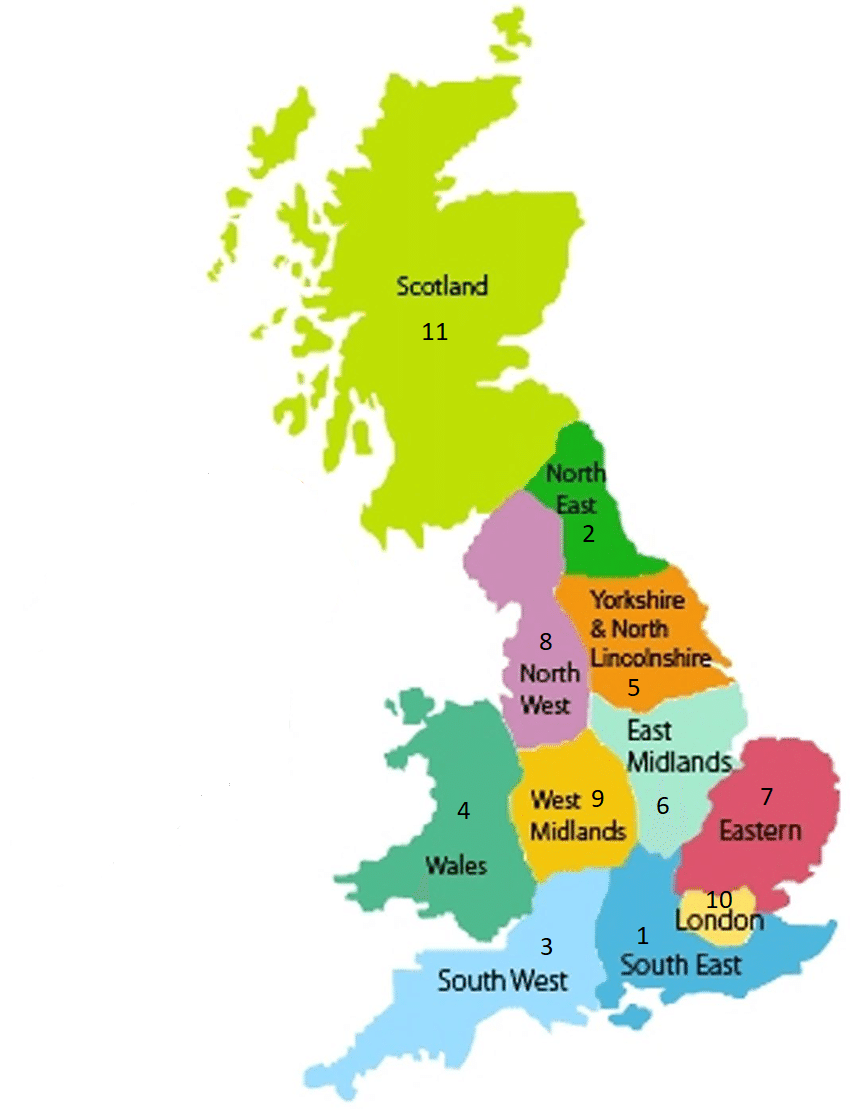
\includegraphics{GOR.png}
\caption{pic\_gov}
\end{figure}

The baseline and the other two areas with a weight close to zero are
Scotland, London and the West Midlands. Scotland and London are prime
candidates to be categories of their own, as Scotland has a strong
regional identity and London is the capital of the country. From a
data-driven perspective, combining the West Midlands with any region
other than London or Scotland does not make sense, as the weight
difference between those region and all other regions is relatively big.
From a theory-driven perspective, we cannot think of any good reason to
combine the West Midlands with London or Scotland: it is not filled with
cities nor is it close enough to Scotland to assume a similar
population.

When assuming that the regions with a near-identical weight are in the
same group and Scotland and London are two seperate categories, only a
few possible groupings remain:

\begin{enumerate}
\def\labelenumi{\arabic{enumi}.}
\tightlist
\item
  South East, South West, and North East England are the third category,
  with Wales and the rest of England being the last category.
\end{enumerate}

\begin{itemize}
\tightlist
\item
  This makes some sense theoretically: the three are the very north and
  south of England, with the remainder being in the middle. Weight-wise
  however, combining the West Midlands with the areas with far lower
  weights does not make sense.
\end{itemize}

\begin{enumerate}
\def\labelenumi{\arabic{enumi}.}
\setcounter{enumi}{1}
\tightlist
\item
  The same as above, but with the West Midlands grouped with London.
\end{enumerate}

\begin{itemize}
\tightlist
\item
  This is more logical weight-wise than the first option, but from a
  theoretical perspective it is strange to combine the city with a rural
  area.
\end{itemize}

\begin{enumerate}
\def\labelenumi{\arabic{enumi}.}
\setcounter{enumi}{2}
\tightlist
\item
  The North West, West Midlands and East of England are the third
  category, with Wales and the rest of England being the last category.
\end{enumerate}

\begin{itemize}
\tightlist
\item
  Weight-wise it is just as logical or illogical as the first option,
  but from a theoretical standpoint taking three areas in the middle
  seems to have less of a basis than taking the outer areas like is done
  in the first option.
\end{itemize}

\begin{enumerate}
\def\labelenumi{\arabic{enumi}.}
\setcounter{enumi}{3}
\tightlist
\item
  The West Midlands alone being the third category, with the rest of
  England being the fourth.
\end{enumerate}

\begin{itemize}
\tightlist
\item
  This fits weight-wise, but why the West Midlands should be taken
  seperately is a mystery. It is however less absurd than combining it
  with London: the West Midlands may have unique features that we do not
  know about, but we do know that it is not a capital like London.
\end{itemize}

In conclusion, the fourth option seems the most likely, as the grouping
is logical from a data-driven perspective and while it does not quite
make sense theoretically, there is no obvious reason to assume that it
is incorrect. The best alternative is the first option, as it makes the
most sense from a theoretical perspective.


\end{document}
